\begin{sfragment}{Setting up the \sTeX IDE}
  
    The \sTeX IDE consists of two components using the 
    \emph{Language Server Protocol (LSP)}: A \emph{client}
    in the form of a VSCode extension, and a \emph{server}
    included in the \mmt system. Installing the extension will
    open up a setup routine that will guide you through the rest.
  
    \begin{sfragment}{The \sTeX VSCode Extension}
  
      If you have not already, you should first install the VSCode editor 
      available at \url{https://code.visualstudio.com/}.
  
      Next, open VSCode and install the \sTeX extension by clicking on
      the \emph{extensions} menu on the very left of the VSCode window
      and searching for ``sTeX'' in the 
      \emph{``Search Extensions in Marketplace''} field, as in
      \autoref{fig:install}, and clicking the \emph{Install}-button
      of the \sTeX extension by KWARC.
  
      \begin{figure}
        \begin{center}
          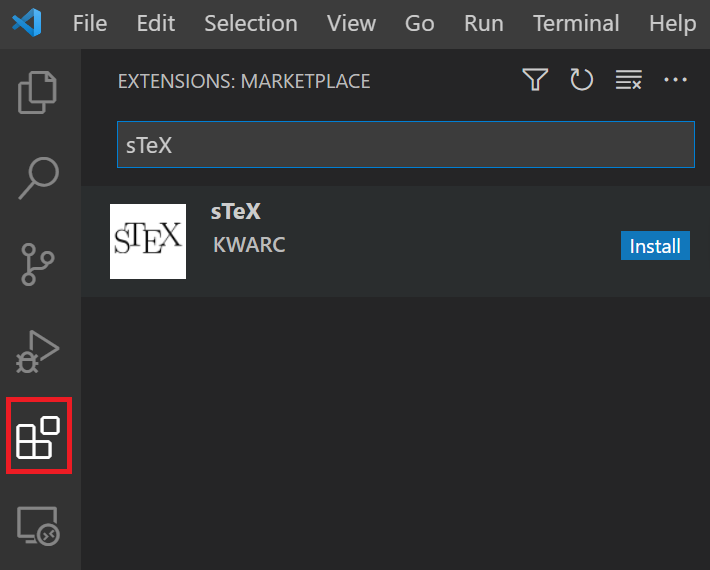
\includegraphics[width=0.6\textwidth]{img/vsc1.png}
        \end{center}
        \caption{Installing the \sTeX extension for VSCode}\label{fig:install}
      \end{figure}
  
    \end{sfragment}
  
    \begin{sfragment}{Setting up \mmt}
  
      Next, open any directory (\texttt{File $\to$ Open Folder...}) that contains
      a \verb|.tex|-file, and a setup window as in \autoref{fig:setup} 
      will pop up. Clik on the highlighted link `\emph{here}' and download
      the latest version of the \texttt{MMT.jar} file (at least version 23.0.0)
      anywhere you like. Then click the \emph{``Browse...''}-button
      and select your freshly downloaded \texttt{MMT.jar}.
  
      If you have already set a system variable for your MathHub-directory,
      you are now done and can click \emph{``Finish''}. If you have not,
      you can now also enter a directory path in the lower text field,
      and the VSCode extension will attempt to globally set one up
      for you, depending on your operating system.
  
      \begin{figure}
        \begin{center}
          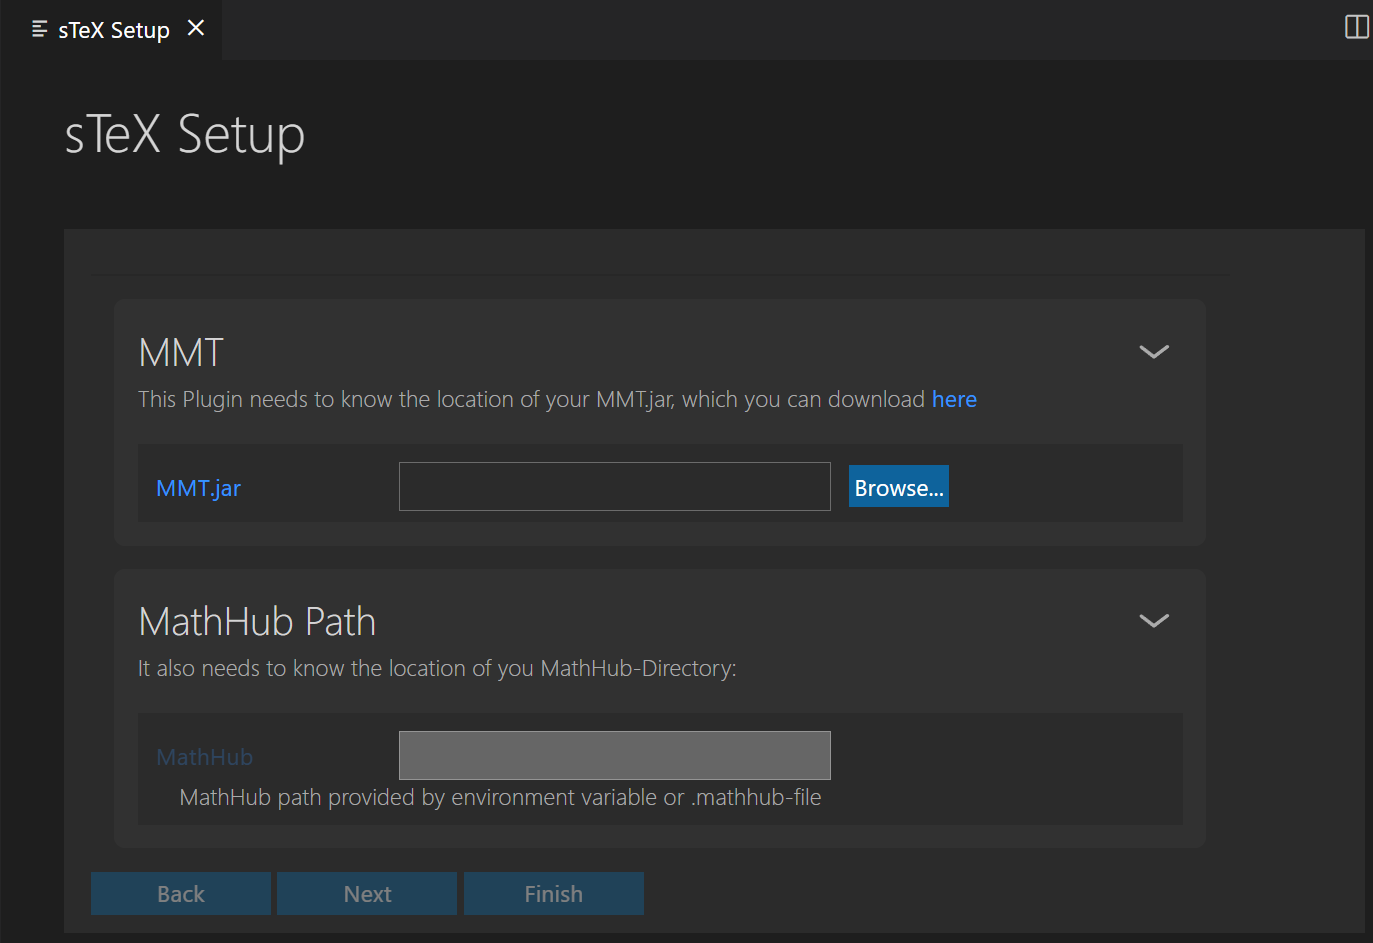
\includegraphics[width=\textwidth]{img/vsc2.png}
        \end{center}
        \caption{\sTeX Setup Routine}\label{fig:setup}
      \end{figure}

      Once you click \emph{``Finish''}, the client will connect
      to \url{https://stexmmt.mathhub.info/:sTeX}, query for
      available archives, download the core libraries required
      for all (or most) semantic services (\texttt{MMT/urtheories}
      and \texttt{sTeX/meta-inf}) and set up \RusTeX for you 
      automatically.
  
    \end{sfragment}
  
  \end{sfragment}